%Préambule du document :
\documentclass[11pt]{article}
\usepackage[utf8]{inputenc}
\usepackage[french]{babel}
\usepackage{amsmath}
\usepackage{tikz}

%Corps du document :
\begin{document}
  \center 
\includegraphics[width=8cm]{logo.png}

\begin{center}
\textsc{\Large M1 Informatique - Projet ANDROIDE}\\[0.5cm]
\textsc{\Large  Carnet de bord }\\[0.5cm]
\textbf{Robotique adaptative en essaim: effet de l'environnement sur l'apprentissage de stratégies collectives} \\[3cm]
\end{center}


\begin{center}
Roza Amokrane\\[0.3cm]
Nabila Ould Belkacem\\[0.8cm]
\textbf{Encadrant:}\\
Nicolas Bredeche \\[0.4cm]
\end{center}


\newpage
\tableofcontents
\newpage

\begin{flushleft}
\section{Introduction}
 Embodied Evolutionary Robotics (EER) est la conception d’algorithmes d'apprentissage distribués en ligne implémentés  sur un groupe de robots. Dans notre projet on s'intéresse dans un premier temps à l'apprentissage de la spécialisation dans un essaim de comportement.Pour cela, on se met dans un environnement où on dispose de deux ressources .Les agents doivent se déplacer et collecter ces ressources afin de survivre. Chaque agent est capable de synthétiser de l'énergie à partir d'une seule ressource determinée par son génome.Chaque ressource suffit pour la survie de la moitié de la population .Donc , pour la survie de la population, la moitié de la population doit d se spécialiser dans une ressource et l'autre moitié dans l'autre ressource.On cherche à comprendre les différents paramètres qui peuvent affecter l'apprentissage. On passera ensuite au cas de l'apprentissage de la coopération .

\section{Les mots clés retenus}

 \begin{itemize} \item Ressource   \item Graphe  \item Agent\item Génome \item Fitness   \item Algorithme de sélection de génome  \item Fitness-prop \item Rank-prop  \item VaNILLA-ELITIST  \item VaNILLA-NOFITNESS 
  \end{itemize} 
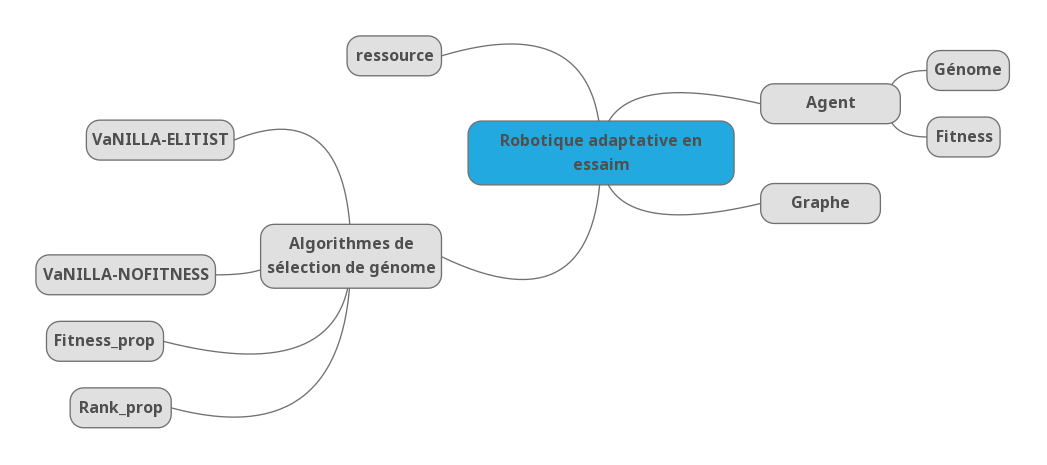
\includegraphics[scale=0.4]{carte.png} 

\section{Descriptif de la recherche documentaire}
   On a commencé notre recherche  par regarder les vidéos et les TDS  qui nous ont  permis de trouver les différents outils de recherche .Puis on a  lu  les articles fournis par notre encadrant pour  comprendre le sujet , ce qui  nous a aidé à déterminer  les mots clés .Par la suite on a utilisé Wikipédia pour comprendre ces mots clés  en langue française et anglaise .On s’est basé aussi sur le moteur de recherche Google permettant d’accéder à des pages web  à partir des mots clés ,titres et des questions qu’on se posait lors de notre recherche.On a utilisé aussi des outils académiques dans le domaine de la science et technologie tel que <web of science> ou on s’est inspiré des articles scientifiques,des livres et des synthèses  bibliographiques écrites par des chercheurs qu'on peut sélectionner par plusieurs critères (date,auteur et type...)
   
     Nous avons déduit que les articles scientifiques et académiques ont un niveau de spécialisation très élevé ,ils sont écrit par de chercheurs qui maîtrisent leurs domaines contrairement  aux outils de vulgarisation qui sont rédigés par des journalistes ou des vulgarisateurs qui ont une connaissance moins profonde du thème .
\section{Bibliographie produite dans le cadre du projet}

\end{flushleft}
\end{document}
